\chapter{Completed Work}\label{sec:completed_work}

\section{Transfemoral Prosthesis Design}\label{sec:completed_design}
\begin{marginfigure}[1.25in]
    \centering
    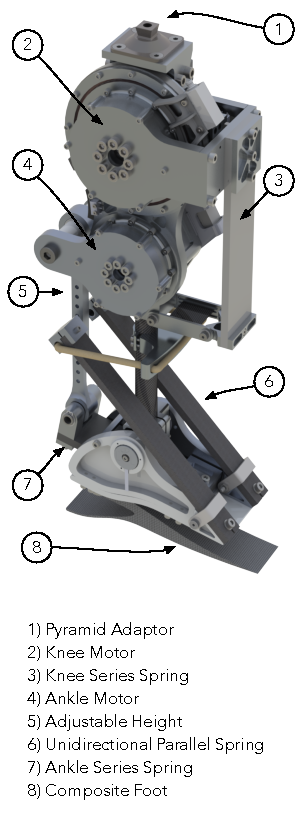
\includegraphics[width=\linewidth]{prosthesis_render_annotated}
    \caption{Render of proposed powered knee and ankle prosthesis design. The
    prosthesis includes series elastic actuators to enable accurate torque
    control and a unidirectional parallel ankle spring to offset the required
    angle torque.}\label{fig:prosthesis_render_annotated}
\end{marginfigure} 

To test our proposed Neuromuscular control approach, and its ability to help
subjects maintain or recover their balance, we build a custom transemoral
prosthesis capable of reproducing dynamic locomotion tasks. The proposed design,
shown in \cref{fig:prosthesis_render_annotated}, uses brushless electric motors
coupled to harmonic drive gear sets to drive both the knee and ankle joints.
Additionally, the joints employ series elastic actuation to enable accurate
torque control and to protect the Harmonic Drive gear sets from sudden impacts.
The design also features a unidirectional parallel spring in the ankle that
partly offsets the torque demands on the ankle motor.  We design both joints to
meet the demands of dynamic locomotion tasks such as running and trip recovery.

The overall design concept sits in a niche between low powered prostheses
designed with commercial applicability in mind
\citep{sup2007design,sup2009preliminary,lawson2014robotic,rouse2015design,
martinez2011antagonistic} which feature onboard actuation and power sources, and
high-powered tethered systems \citep{caputo2013experimental,
caputo2015informing} with off board actuation designed exclusively for use in
lab environment. Our design features onboard actuators that are more powerful
than those used in standalone devices, but less capable than those employed in
tethered devices. To ensure a reasonable overall weight the device's batteries,
motor drivers, and computers are off board. With this design, we expect to be
able to test control ideas without encountering hardware performance limitations
as with a tethered device. At the same time the device is capable of functioning
outside of the lab environment like a standalone prosthesis. 

\begin{table}
    \centering
    \begin{tabular}{lcc}
        \toprule
        Specification         & Desired Value & Achieved Value \\
        \midrule                  
        Maximum Knee Torque   & $\unit[160]{N \cdot m}$ 
            & $\unit[170]{N \cdot m}$   \\
        Maximum Knee Speed    & \unitfrac[1.80]{rev}{s} 
            & \unitfrac[1.93]{rev}{sec} \\
        Maximum Ankle Torque  & $\unit[200]{N \cdot m}$ 
            & $\unit[170 \ (+120^*)]{N \cdot m}$ \\
        Maximum Ankle Speed   & \unitfrac[1.14]{rev}{s} 
            & \unitfrac[1.22]{rev}{s} \\
        Weight                & \unit[6.8]{kg} & \unit[5.9]{kg} \\
        Minimum Height        & \unit[42.5]{cm} & \unit[42]{cm} \\
        \bottomrule
    \end{tabular}
    \caption{Designed and achieved design specifications. ($^*$Maximum total
    ankle torque is $\unit[290]{N \cdot m}$ achieved at \unit[10]{degrees} of
    dorsiflexion.)}\label{tab:pros_requirements}
\end{table}

\Cref{tab:pros_requirements} shows the desired design specifications for the
transfemoral prosthesis and the values achieved by the final design. To obtain
these design specifications we examined a number of studies that elicited trip
responses.

We specify desired joint torque and speed values to meet the requirements of
demanding tasks such as running. The maximum knee torque specification comes
from the findings of \citet{whitley2008maximum}, who tested the joint torques
used during recovery from a simulated fall. The maximum knee speed requirement
comes from \citet{grabiner1993kinematics}, who tested subjects' responses to
simulated trips induced by unseen obstacles on a walkway. We obtain the maximum
ankle torque requirement from \citet{pijnappels2005early}, who tripped subjects
using a obstacles that could suddenly emerge through the floor. The maximum
ankle speed requirement comes from the running data of
\citet{novacheck1998biomechanics}. We set to the minimum height specification,
measured between the center of the knee and bottom of the foot, to accommodate
the $10^\tn{th}$ percentile female \citep{gordon1988anthropometric}.  Finally,
the required weight corresponds to the mean leg weight of a $50^\tn{th}$
percentile male \citep{winter2009biomechanics}.

\subsection{Knee Joint}
\begin{comment}
\begin{marginfigure}[0in]
    \centering 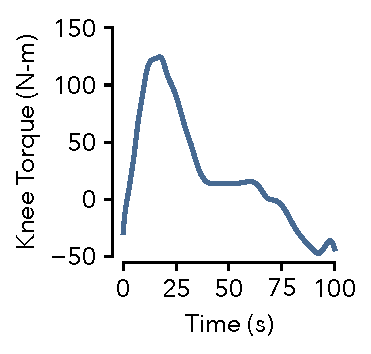
\includegraphics[width=\linewidth]{knee_running_torque}
    \caption{Knee torque required for running}\label{fig:knee_running_torque}
\end{marginfigure}
\begin{marginfigure}[0in]
    \centering 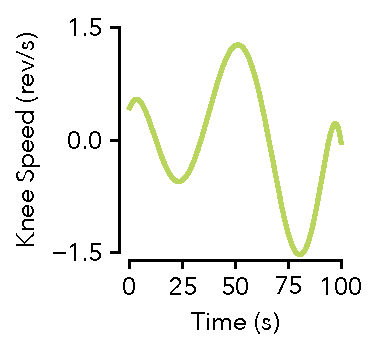
\includegraphics[width=\linewidth]{knee_running_speed}
    \caption{Knee torque required for running}\label{fig:knee_running_speed}
\end{marginfigure}
\end{comment}

In addition to achieving the maximum speeds and torques found in
\cref{tab:pros_requirements}, we design the knee joint so that it can reproduce
the torque and speed required for a \unit[80]{kg} person to run at
\unitfrac[3.2]{m}{s} as measured by \citet{novacheck1998biomechanics}. To
reproduce this trajectory in the knee joint, we utilize a RoboDrive ILM
$85\times13$ HS-SP motor coupled to a Harmonic Drive Gear set with a 50:1
reduction (CSG--25--50). \Cref{fig:knee_motor_torque} shows the motor torque
and speed required to reproduce a running trajectory assuming a gear
efficiency of $75\%$. In this plot, we see that the running trajectory lies
within the speed-dependent torque limit of the motor. Moreover, the root mean
squared torque of this trajectory $(\unit[1.46]{N \cdot m})$ exceeds the torque
rating of the motor $(\unit[1.43]{N \cdot m})$ by just $2\%$. Therefore, the
knee joint should be able to provide the necessary torque to enable running for
a short amount of time, or continuously for lighter subjects or at a slightly
reduced speed.
\begin{marginfigure}[-2in]
    \centering 
    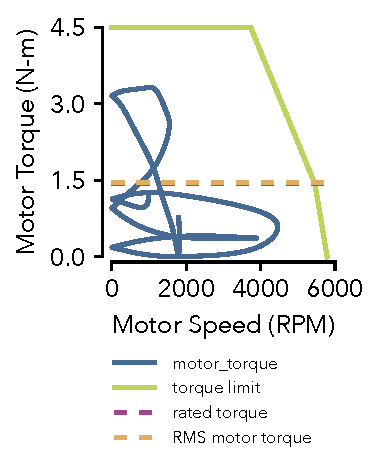
\includegraphics[width=\linewidth]{knee_motor_torque}
    \caption{Knee motor torque required for
    running}\label{fig:knee_motor_torque}
\end{marginfigure}

\begin{figure*}[t]
    \centering 
    \includegraphics[width=\linewidth]{knee_design}
    \caption{Internal and external design of the knee 
    joint.}\label{fig:knee_design}
\end{figure*}
\Cref{fig:knee_design} shows the internal and external design of the knee joint.
The primary component in the knee joint is the stator housing. On top of the
housing is a standard pyramid adaptor that allows the prosthesis to connect to
amputee's sockets. Within the stator housing, lies the brushless motor stator,
rotor, and harmonic drive gear set. We sense absolute rotor angle for
commutation of the brushless motor via hall effect sensors and a magnetic
complementary sin/cos encoder. To incorporate series elasticity, we take
inspiration from the design of the bipedal robot Atrias
\citep{grimes2013atrias}, which uses fiberglass series leaf springs. In our
design, the output of the gear set drives the proximal end of a fiberglass leaf
spring in series with the shank. Two Renishaw Resolute absolute encoders measure
the deflection of this spring to enable torque control.

In addition to allowing for accurate torque control, as shown by
\citet{au2007biomechanical,au2008powered}, the series elasticity also plays a
crucial role in protecting fragile gear components from impact loads. To choose
the spring stiffness for the knee joint, we simulate the prosthesis impacting a
rigid wall with the foot during swing. To do this, we construct a model of the
prosthesis in Matlab Simulink Simulink Simscape Multibody that includes the
series elasticity, gear dynamics, and motor electrical dynamics (for
details see \cref{sec:sec_simulation_environ}). \Cref{fig:impact_sim_knee} shows
the simulation environment. The prosthesis is attached to the distal end of a
thigh segment with a fixed hip position. We control the hip via the ideal swing
leg control outlined in \cref{sec:neuro_ideal_swing} (\cref{eq:hipfeedback}) and
consider the case where the external voltage applied to the motor is zero. This
simulation suggests that a spring stiffness under $\unitfrac[2300]{N \cdot
m}{rad}$ will ensure that the peak impact torque remains lower than the peak
allowable impact torque of the Harmonic Drive of $\unit[242]{N \cdot m}$.
\begin{marginfigure}[-2.5in]
    \centering 
    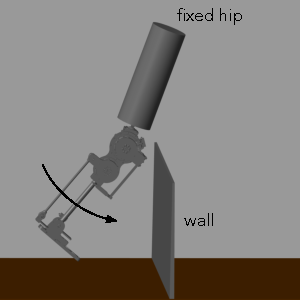
\includegraphics[width=\linewidth]{knee_impact_sim}
    \caption{Impact simulation we used to determine appropriate series spring
    stiffness.}\label{fig:knee_impact sim}
\end{marginfigure}

\subsection{Ankle Joint}
In the ankle joint we utilize a RoboDrive ILM $70\times10$ HS-SP motor coupled
to a Harmonic Drive Gear set with a 100:1 reduction (CSG--20--100). As with the
knee joint, we design the ankle joint to satisfy the requirements listed in
\cref{tab:pros_requirements}. Specifically, for the ankle joint we pay
considerable attention to the tripping condition described by
\citet{pijnappels2005early}, in which the ankle generates a peak torque of
$\unit[202]{N \cdot m}$. 

\begin{marginfigure}[-0in]
    \centering 
    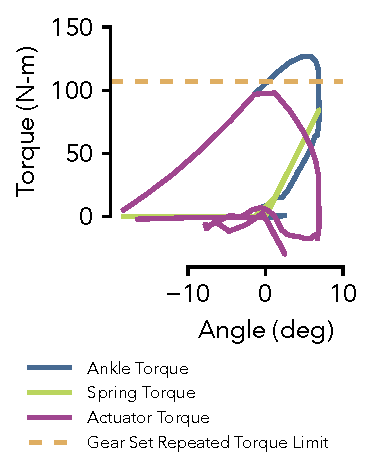
\includegraphics[width=\linewidth]{ankle_torque_vs_angle_ups}
    \caption{Ankle torque vs angle curve during steady, level-ground walking
    (blue) (\citet{winter2009biomechanics} scaled to \unit[80]{kg} person). A
    unidirectional parallel spring can provide a portion of this torque (green)
    and reduces the required actuator torque (purple) to lie under repeated
    torque limit of the Harmonic Drive Gear set (orange).
    }\label{fig:ankle_torque_vs_angle_ups}
\end{marginfigure}
To avoid using a large and heavy motor to achieve this peak torque, we take
inspiration from previous prosthetic ankle designs that employ a unidirectional
parallel spring in the ankle joint that performs the conservative portion of the
ankle's torque versus angle trajectory during normal walking
\citep{au2007biomechanical,au2008powered,sup2009preliminary,lawson2014robotic}.
The parallel spring offsets the required motor torque, as the actuator only
needs to provide the difference between the desired torque and the torque
provided by the parallel spring. \Cref{fig:ankle_torque_vs_angle_ups} shows the
torque versus angle curve during level ground walking
(\citet{winter2009biomechanics}, scaled to \unit[80]{kg} person). In green we
show the torque generated by a $\unitfrac[700]{N \cdot m}{rad}$ parallel spring
optimized to minimize the root-mean-squared motor torque for this trajectory.
From this plot, we see that with the parallel spring, the peak torque is lower
than the repeated peak torque limit of the Harmonic Drive Gear set.
\begin{figure}[b]
    \centering 
    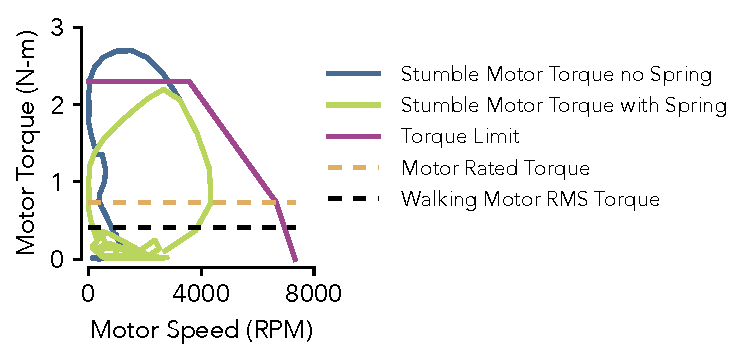
\includegraphics[height=2in]{ankle_motor_torque_tripping}
    \caption{Ankle motor torque required to take the trip recovery action
    observed by \citet{pijnappels2005early} (blue, trajectory obtained by
    scaling walking data from \citet{winter2009biomechanics} to a peak torque of
    $\unit[202]{N \cdot m}$, $75\%$ gear efficiency assumed). Using a parallel
    spring allows the motor to produce the required torque (green) while
    remaining within it's torque limit (purple).
    }\label{fig:ankle_motor_torque_tripping}
\end{figure}

The tripping data obtained by \citet{pijnappels2005early} shows that the ankle
kinematics during trip recovery are similar to those seen during normal walking.
Therefore, the parallel spring, should be able to contribute torque during the
tripping case as well. To confirm this, \cref{fig:ankle_motor_torque_tripping}
shows the motor torque required for trip recovery (obtained by scaling walking
torque data from \citet{winter2009biomechanics} to have a peak torque of
$\unit[202]{N \cdot m})$ We see that the inclusion of the parallel spring allows
the prosthesis to produce enough net torque to reproduce the trip recovery
trajectory without exceeding the torque limit of the motor. 

Finally, \cref{fig:ankle_motor_torque_running} shows the torque and speed
required of the motor for running \citep{novacheck1998biomechanics}. In this
case, we use an ankle parallel stiffness of $\unitfrac[267]{N \cdot m}{rad}$.
From this plot, we see that this combination of ankle motor and spring is nearly
sufficient for running. Increasing the voltage of the prosthesis from
\unit[48]{V} to \unit[60]{V} or decreasing the gear ratio from 100:1 to 80:1
will allow the torque trajectory to fit completely within the motor limits. 
\begin{marginfigure}[-0in]
    \centering 
    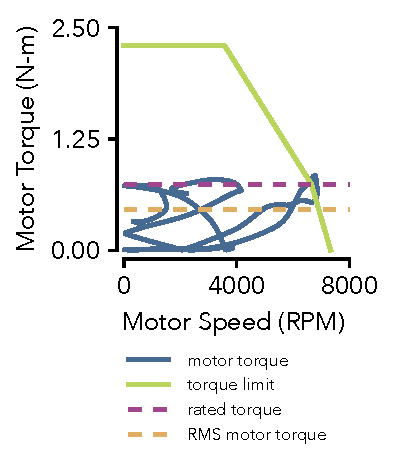
\includegraphics[width=\linewidth]{ankle_motor_torque_running}
    \caption{Ankle motor torque required to reproduce the running trajectory
    recorded by \citet{novacheck1998biomechanics} assuming a parallel spring
    stiffness of $\unitfrac[267]{N \cdot m}$ and a gear efficiency of $75\%$.
    }\label{fig:ankle_motor_torque_running}
\end{marginfigure}

\Cref{fig:ankle_design} shows an internal view of the ankle actuator and
external views of the actuator and foot mechanism. In the ankle design, the
output of the actuator actuates the foot through a four-bar mechanism. The
actuator pulls or pushes on the proximal end of a length-adjustable tendon. The
distal end of the tendon attaches to one end of a fiberglass series elastic leaf
spring that is also connected to the foot. By measuring the angles of the ankle
actuator output and the ankle joint and using the equations of the four-bar
mechanism's kinematics, we can calculate the deflection of the leaf spring and
thus the torque applied to the ankle.
\begin{figure*}[b!]
    \centering 
    \includegraphics[width=\linewidth]{ankle_design}
    \caption{Internal and external design of the ankle 
    joint.}\label{fig:ankle_design}
\end{figure*}

The design of the ankle actuator represents a second iteration of the knee
actuator design and features two main improvements.  First, it has increased
space on the side of the motor for cable routing. Second, the ankle actuator has
a solid rotor shaft. In contrast, the knee actuator's shaft is comprised of two
parts: one that held the motor rotor and transferred power through the gear set,
and another that held the sin/cos encoder's magnetic shaft component. In
practice, these two components proved difficult to align, causing degraded
performance of the sin/cos encoder. The ankle actuator's solid shaft ensures the
encoder magnet stays aligned with the read head.

\begin{marginfigure}[-0.0in]
    \centering 
    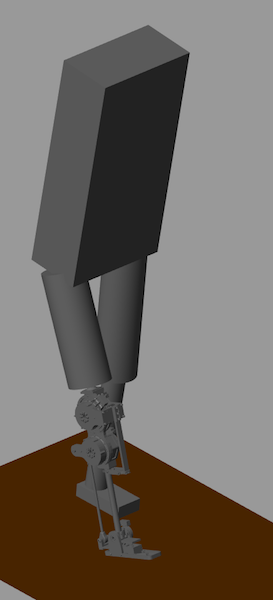
\includegraphics[height=2in]{ankle_impact_sim}
    \caption{Impact simulation we used to determine appropriate series spring
    stiffness.}\label{fig:ankle_impact_sim}
\end{marginfigure}
As with did for the knee series spring, we again determine an acceptable ankle
spring stiffness by performing an impact simulation. For the ankle, we simulate
an \unit[80]{kg} person stepping on the prosthesis when the motor driver
provides the ankle motor with zero applied voltage. \Cref{fig:ankle_impact_sim}
shows the simulation environment. From this simulation we find that a spring
stiffness of about $\unitfrac[1000]{N \cdot m}{rad}$ should sufficiently protect
the ankle gear set from impacts. This estimate is likely softer than necessary
due to the additional series compliance in the amputee's socket and the
composite foot that are not included in the simulation.

\subsection{Experiments on Powered Knee/Passive Ankle Prosthesis}
Towards a full realization and study on amputee subjects, we present a partial
implementation and evaluation of the control on the current prosthesis prototype
worn by a non-amputee user. \Cref{fig:test_bed_annotation} shows an able-bodied
user wearing our current prosthesis prototype. The current prosthesis prototype
has an active knee SEA unit and an unpowered, spring-loaded, ankle.  We connect
the prosthesis to a knee crutch (iWalk 2.0 Hands Free Crutch) in order to allow
a non-amputee experimenter to test the control. Additionally, the experimenter
wears a lift shoe to compensate for the added thigh length of the knee crutch
and prosthesis.
\begin{figure}
    \centering 
    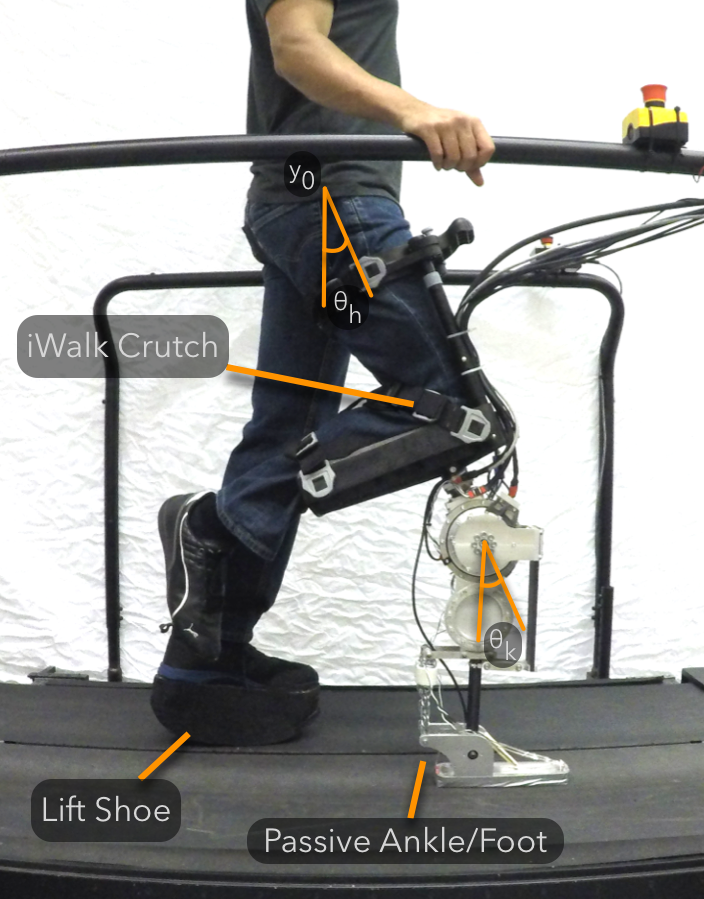
\includegraphics[height=3in]{test_bed_annotation}
    \caption{A non-amputee experimenter tests the prosthesis using an iWalk
    Crutch as a knee adaptor. The experimenter wears a lift shoe on the
    contralateral leg to compensate for the added thigh length of the prosthesis
    and knee adaptor.
    }\label{fig:test_bed_annotation}
\end{figure}

To control the prosthesis knee, we use Simulink Real-Time (Mathworks, USA),
which samples all sensors (joint encoders, IMU on thigh, force sensors in foot),
runs a velocity-based SEA control \citep{schepelmann2012development}, and sends
commands to the motor controller at a rate of 1kHz. Given a desired torque,
$\tau_d$, and a measured torque error, $\tau_e$, the commanded motor velocity is
given by
\begin{align}
    \omega_m = \frac{1}{k} \frac{\tn{d} \tau_d}{\tn{d} t} + \omega_l 
        + \func{PD}{\tau_e},
\end{align}
where $\omega_l$ is the velocity of the load-side of the series spring (the
shank) and $\func{PD}{\cdot}$ is a proportional-derivative feedback term. 

The behavior control of the knee is a hybrid model that combines the
Neuromuscular Stance control described in \cref{sec:neuro_stance_reflexes} with
the idealized swing control outlined in \cref{sec:neuro_ideal_swing}. The
missing ankle actuation in the current prosthesis prototype restricts the
neuromuscular stance control to those muscles that span the knee: the vastus,
hamstring, and gastrocnemius. The hamstring and vastus are stimulated according
to \cref{eq:ham_stim_full,eq:vas_stim_full} respectively.  Similarly, the
gastrocnemius is stimulated by positive force feedback. (The torso balance
contribution of the complete hamstring stimulation, \cref{eq:ham_stim_full}, is
neglected.) The realtime software executes the hybrid neuromuscular behavior
control at a rate of 5kHz, ensuring that the integration (ode1) of the simulated
muscle dynamics remains stable. During swing, we only use the knee portion of
the swing control given by \crefrange{eq:flexphase}{eq:extend}. In late swing,
the control transitions between the two phases in proportion to the measured
ground reaction force (\cref{eq:stance_grf_trans,eq:swing_grf_trans}).

% Generation of normal stance behavior
\subsection{Slow Walking Behavior}
We first test if the prosthesis control can reproduce normal stance and swing
behavior of the lower limb in steady-state walking. For this purpose, we capture
joint kinematics and kinetics as well as the virtual muscle activations of the
prosthesis control while an experimenter walks for ten trials with the crutch
and prosthesis system on a treadmill. Because the fit of the crutch to the
experimenter's leg is not very tight, we limit the walking speed to
\unitfrac[0.5]{m}{s} and the experimenter holds onto handrails for safety
(\cref{fig:test_bed_annotation}).
\begin{figure}[t]
    \centering
    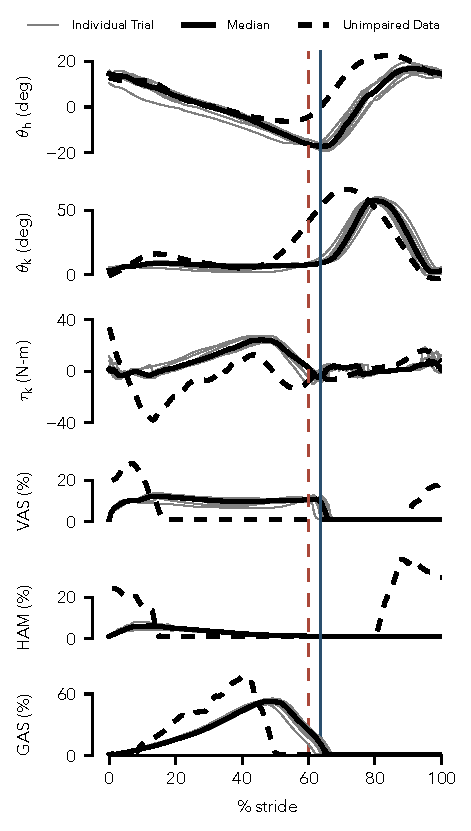
\includegraphics[width = 3in]{pros_gait_data}
    \caption{Prosthesis behavior at walking speed of 0.5 m/s. Shown are the hip
    and knee trajectories, the knee controller torque, and the activations of
    the vastus, hamstring, and gastrocnemius muscles generated by the
    prosthesis control in the testbed. Solid black lines show averaged data  of
    ten trials with the individual trials depicted in gray. Dashed lines show
    corresponding data from human walking at preferred speed (joint angles and
    knee torque: \citet{winter2009biomechanics}, muscle surface
    electromyograms: \citet{perry2010gait}). Solid and dashed vertical lines
    indicate median toe off times for the prosthesis and human data
    respectively.
    }\label{fig:pros_gait_data}
\end{figure}

The control generates steady-state prosthesis behavior that qualitatively
reproduces human leg behavior in walking. \Cref{fig:pros_gait_data} compares the
observed prosthesis leg behavior (solid lines) to corresponding human data at
preferred walking speed (dashed lines, adapted from
\citet{winter2009biomechanics,perry2010gait}). The hip and knee kinematics match
overall, although later transitions from stance to swing are observed in both
joints ($\theta_h$ and $\theta_k$) and the prosthesis knee flexes less in stance
($\theta_k$). The knee torque follows trends similar to human data, but the peak
flexion and extension torques in the early stance phase are diminished
($\tau_k$). These lower peaks are caused by reduced activations of the virtual
vastus and hamstring muscles (VAS and HAM) in this phase, a clear difference to
these muscles' activation in humans, in which bursts of activity at heel strike
are followed by relative silence. Finally, the activity of the virtual
gastrocnemius muscle (GAS) bears strong similarity the activity of this muscle
in human walking.

To some extent, limitations of our current experimental testbed may
account for observed discrepancies. The imposed slow walking speed of 0.5 m/s
required less energy absorption in early stance than at normal walking speed.
Moreover, the experimenter held onto the handrails to assist with lateral
balance, which may have channeled some impact energy through the arms. In
addition, the hybrid nature of the proposed control prevents the virtual
muscles from activating in swing, which is the case in humans
(\cref{fig:pros_gait_data}, VAS and HAM activities from 80\% to 100\% of gait
cycle), and would alter the response of the virtual muscles at heel strike.
Finally, the lack of an active ankle and its control in the current prosthesis
prototype further limits how closely the leg behaviors can match.

% Response to Swing Leg Tripping
\subsection{Response to Swing Leg Tripping} 

In a second set of experiments, we evaluate the response of the prosthesis
controller to trip disturbances. We apply disturbances during treadmill walking
by commanding flexion knee torques to the prosthesis in addition to its
swing-leg control torque. The added torque simulates an obstacle encounter
modeled in the same way as the stopping torque of the swing leg control,
\cref{eq:stop}, with $\alpha_{thr}$ replaced by a disturbance leg angle. The
foot can pass the simulated obstacle if the leg length contracts beyond a
threshold of \unit[94]{cm}. For an early-, mid-, or late-swing encounter, the
disturbance angle is set to 110, 95, or \unit[80]{degrees}, respectively. In
addition, anticipation of the trip by the experimenter is prevented by applying
the disturbance only with a probability of 25\%.

\begin{figure}[b!]
    \centering
    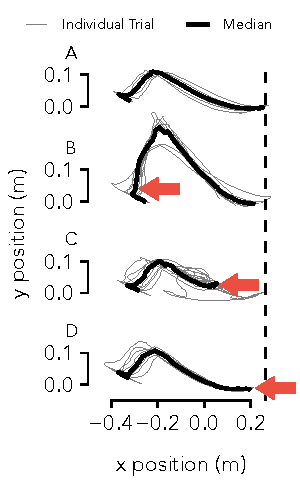
\includegraphics[width = 3in]{impulse_hardware_annotated}
    \caption{Response to simulated tripping disturbance. (A) Undisturbed ankle
    trajectory calculated from hip and knee angles assuming constant hip height.
    (B-D) Ankle trajectories with disturbance applied in early, mid and late
    swing (arrows). The vertical dashed line shows the target landing position
    of the foot, which corresponds to a \unit[75]{degree} landing angle.}
    \label{fig:impulse_hardware}
\end{figure}

The experiments reveal that in response to disturbances during early and late
swing, the prosthesis control places the swing leg with high repeatability and
produces leg elevating and lowering strategies observed in humans.
\cref{fig:impulse_hardware} shows the Cartesian ankle trajectory in swing over
10 trials for the undisturbed (A) and disturbed conditions (B-D). In the
undisturbed condition, the leg placement is repeatable with an interquartile
range (IQR) of landing positions of \unit[3.1[{cm} and a bias of \unit[2.7]{cm}
(median) from the target (dashed line).  (Further tuning of the control
parameters should improve the landing position accuracy.)

In the early disturbance condition (\cref{fig:impulse_hardware}B), the
prosthesis generates large knee flexion roughly doubling the peak ground
clearance. Nonetheless, the median landing position remains within
\unit[5.3]{cm} of the target (IQR: \unit[10.2]{cm}), demonstrating the knee
control's ability to compensate for early swing disturbances. This response is
similar to the leg elevating strategy observed in humans when disturbed shortly
after toe-off \citep{eng1994strategies, schillings2000muscular}. The biological
strategy, however, shows active knee flexor muscle contributions, while the
prosthesis knee flexion is entirely passive, as the leg angular velocity does
not become negative during the disturbance (Eq.~\ref{eq:flexphase},
\cref{sec:neuro_ideal_swing}).

In the late disturbance condition \cref{fig:impulse_hardware}D),
the prosthesis leg behavior resembles the lowering strategy of
humans~\citep{schillings2000muscular}, in which knee extensor muscles quickly
extend the leg. This behavior is triggered on the prosthesis in the third phase
of the swing control before the leg angle starts to retract
(\cref{eq:extend}). The prosthesis achieves ground contact slightly earlier
with a median landing point of \unit[8.8]{cm} before the target (IQR:
\unit[3]{cm}).

Finally, \cref{fig:impulse_hardware}C shows the response of the
prosthesis to a mid-swing disturbance. When humans are confronted with
disturbances in mid swing, they may use either elevating or lowering strategies
\citep{eng1994strategies, schillings2000muscular}. However, the prosthesis
response resembles neither strategy. During mid swing, the prosthesis control
uses a holding policy, damping both knee flexion and extension
(\cref{eq:holdphase}). Consequently, in most cases the knee angle neither
flexes adequately to clear the obstacle nor extends quickly enough to make
timely ground contact. In these trials, falling was only prevented via support
from the treadmill handrails.

\section{Comparison of Robustness Achieved by Reflex and Impedance Controls in
    Simulation}\label{sec:completed_comparison}

\subsection{Simulation Environment}\label{sec:sec_simulation_environ}

\subsection{Controller Optimization}\label{sec:completed_comparison_opt}

\subsection{Results}\label{sec:completed_comparison_results}

\subsection{Discussion}\label{sec:completed_comparison_discuss}

\section{Optimization of Systems Using
    Preferences}\label{sec:completed_pref_opt}
